\documentclass[10pt]{beamer}
\usetheme{jambro}

\title[]{Pensamento Econômico Contemporâneo - A escola Keynesiana ortodoxa}
\author[]{Paulo Victor da Fonseca}
\date{}

\hypersetup{
    colorlinks = true,
    urlcolor = teal,
    linkcolor = teal    
}
\usepackage[portuguese]{babel}
\usepackage{subfig}
\usepackage{emoji}

\begin{document}

\begin{frame}[plain]
    \titlepage{
        \begin{center}
            \begin{minipage}{0.8\textwidth}
                \centering
            \end{minipage}
        \end{center}}
\end{frame}

\begin{frame}{Sumário}
    \tableofcontents
\end{frame}

\section{Curva de Phillips e economia Keynesiana ortodoxa}
\begin{frame}{Curva de Phillips}
    \begin{itemize}
        \item \textcolor{blue}{Curva de Phillips}: relação entre inflação e desemprego, uma das mais famosas relações em macro
        \bigskip
        \item Em 1958, A.W.Phillips publicou um estudo estatístico investigando a relação entre desemprego ($U$) e a taxa de variação dos salários nominais ($W$) no UK: 1861-1957
    \end{itemize}
\end{frame}

\begin{frame}{Curva de Phillips}
    \begin{figure}
        \centering
        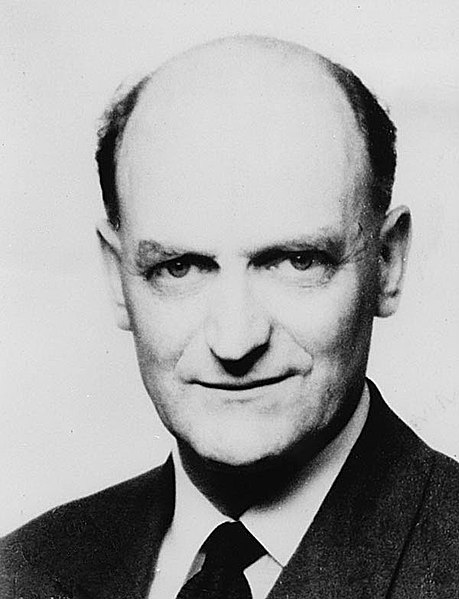
\includegraphics[width=0.3\textwidth]{./figures/aula8_fig1.jpg}
        \caption{Alban William Housego Phillips (1914-1975).}
        \label{fig:phillips}
    \end{figure}
\end{frame}

\begin{frame}{Curva de Phillips}
    \begin{figure}
        \centering
        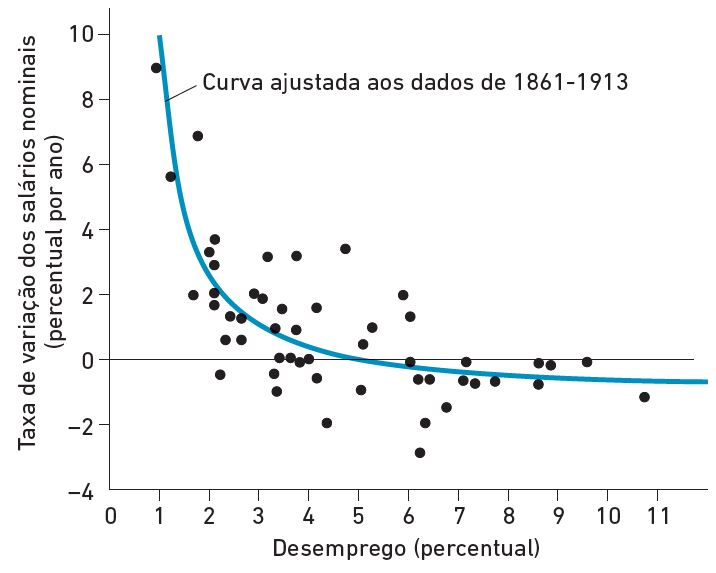
\includegraphics[width=0.5\textwidth]{./figures/aula8_fig2.JPG}
        \caption{A curva de Phillips original - UK. Fonte: Dornbusch et al. (2013).}
        \label{fig10}
    \end{figure}
\end{frame}

\begin{frame}{Curva de Phillips}
    \begin{itemize}
        \item Figura \ref{fig10}: a relação média estimada é não-linear e inversa
        \bigskip
        \item E.g., a um nível de desemprego de $\approx 5,5\%$, a taxa de variação dos salários nominais é 0\%; a um nível de desemprego de $\approx 2,5\%$, a taxa de variação dos salários nominais foi de 2\%
        \bigskip
        \item Relação estimada para 1861-1913:
        \begin{equation}
            \dot{W} = -0,9 + 9,638(U)^{-1,394}
            \label{eq3}
        \end{equation}
    \end{itemize}
\end{frame}

\begin{frame}{Curva de Phillips}
    \begin{itemize}
        \item Phillips verificou que os dados para o período 1948-1957 aproximavam muito bem a curva obtida para o período anterior
        \bigskip
        \item Resultado que sugeria a possível existência de uma relação negativa entre inflação salarial e desemprego \hlight{estável de longo prazo}
    \end{itemize}
\end{frame}

\begin{frame}{Curva de Phillips}
    \begin{itemize}
        \item Phillips: investigação empírica, mas com uma possível explicação teórica para o resultado obtido:\bigskip
        \NB{
            Quando a demanda por um bem ou serviço \'{e} alta relativamente \`{a} oferta, esperamos um aumento de pre\c{c}os, sendo a taxa de varia\c{c}\~{a}o maior quanto maior for o excesso de demanda. Por outro lado, quando a demanda \'{e} baixa relativamente \`{a} oferta, esperamos uma queda de pre\c{c}os, sendo a taxa de varia\c{c}\~{a}o maior quanto maior for a defici\^{e}ncia de demanda. Parece plaus\'{i}vel que este princ\'{i}pio deve operar como um dos fatores determinantes da taxa de varia\c{c}\~{a}o das taxas de sal\'{a}rios nominais.
        \begin{flushright}
            (Phillips, 1958).
        \end{flushright}
    }
    \end{itemize}
\end{frame}

\begin{frame}{Curva de Phillips}
    \begin{itemize}
        \item Pós publicação de Phillips, emergência de uma literatura empírica e uma teórica
        \bigskip
        \item Empírica: verificar se havia uma relação estável entre inflação e desemprego em outras economias de mercado
        \bigskip
        \item Quanto à possibilidade de existência simultânea de baixa inflação e baixo desemprego, a descoberta de um possível trade-off entre esses dois objetivos implicava um dilema de política econômica, que poderia ser resolvido se a curva pudesse ser deslocada para a esquerda com a adoção de políticas econômicas apropriadas
        \bigskip
        \item Design de políticas efetivas para alcançar esse objetivo necessita de um arcabouço teórico coerente que explique as forças econômicas subjacentes à relação observada
    \end{itemize}
\end{frame}

\begin{frame}{Curva de Phillips}
    \begin{itemize}
        \item Lipsey (1960) primeira formulação teórica via combinação de duas relações:
        \bigskip
        \begin{enumerate}
            \item relação positiva e linear entre a taxa de crescimento dos salários nominais e o excesso de demanda por trabalho ($X_L$)
            \medskip
            \item relação negativa e não-linear entre o excesso de demanda e desemprego
        \end{enumerate}
        \bigskip
        \item Formalmente:
        \begin{eqnarray}
            \dot{W} = \alpha(X_L) &=& \alpha[(D_L - S_L)/S_L], \label{eq4} \\
            X_L &=& \beta(U), \label{eq5}
        \end{eqnarray}
        onde $D_L$ é a demanda por trabalho, $S_L$ oferta de trabalho, $\alpha > 0$ um coeficiente de flexibilidade dos salários.
    \end{itemize}
\end{frame}

\begin{frame}{Curva de Phillips}
    \begin{itemize}
        \item $\beta$ é um parâmetro variável negativo tal que quando $X_L \to 0$, $U = U^*$ e $U^*>0$, e quando $X_L \to \infty$, $U \to 0$
        \bigskip
        \item A combinação destes dois postulados forneceu uma justificativa econômica para a relação inversa e não-linear entre taxa de variação de salários nominais e desemprego
    \end{itemize}
\end{frame}

\begin{frame}{Curva de Phillips}
    \begin{figure}
        \centering
        \href{https://raw.githubusercontent.com/pvfonseca/pec/main/notas/figures/aula8_fig3.PNG}{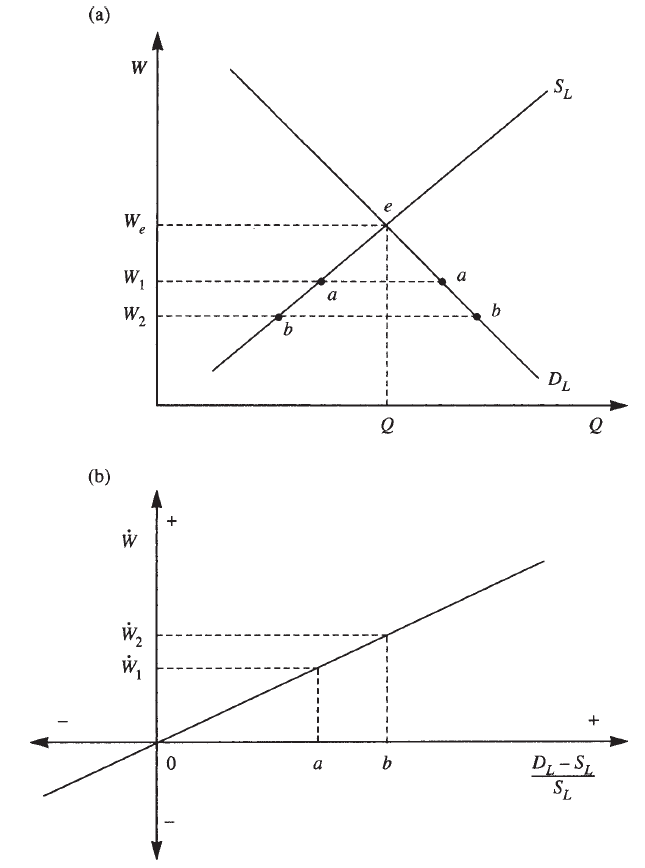
\includegraphics[width=0.3\textwidth]{./figures/aula8_fig3.PNG}}
        \caption{Relação entre variação salarial e excesso de demanda por trabalho. Fonte: Snowdon e Vane (2005).}
        \label{fig11}
    \end{figure}
\end{frame}

\begin{frame}{Curva de Phillips}
    \begin{itemize}
        \item Figura \ref{fig11} ilustra a relação entre variação salarial e excesso de demanda por trabalho
        \bigskip
        \item Painel (a): para qualquer taxa salarial abaixo de $W_e$, os salários irão crescer como resultado do excesso de demanda por trabalho
        \bigskip
        \item Painel (b): a taxa de crescimento será maior quanto maior for o excesso de demanda por trabalho
    \end{itemize}
\end{frame}

\begin{frame}{Curva de Phillips}
    \begin{figure}
        \centering
        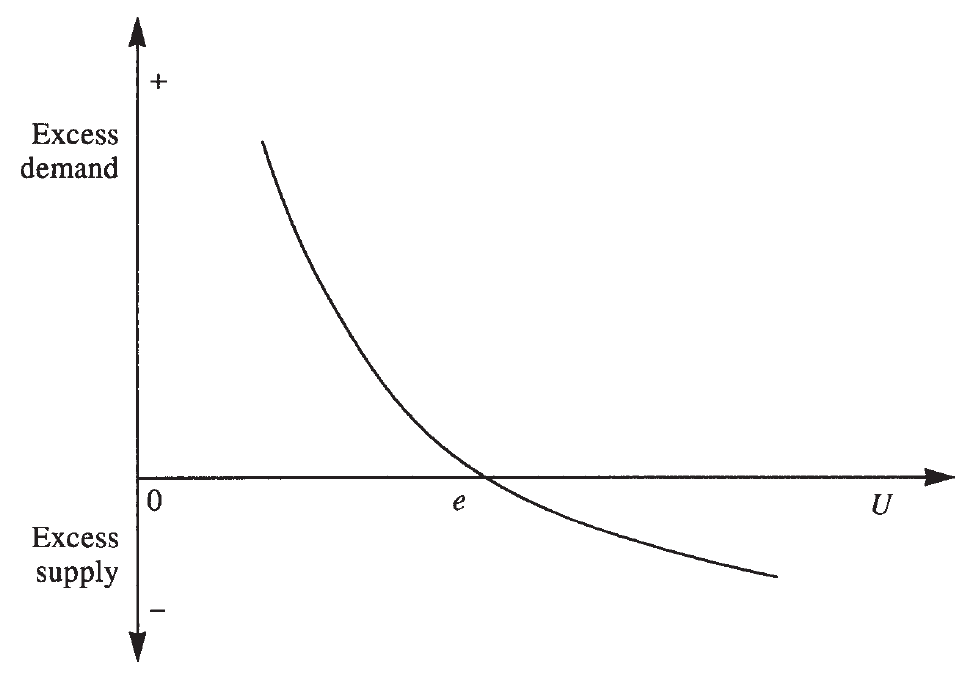
\includegraphics[width=0.6\textwidth]{./figures/aula8_fig4.PNG}
        \caption{Relação entre excesso de demanda por trabalho e desemprego. Fonte: Snowdon e Vane (2005).}
        \label{fig12}
    \end{figure}
\end{frame}

\begin{frame}{Curva de Phillips}
    \begin{itemize}
        \item Figura \ref{fig12}: relação entre excesso de demanda por trabalho e desemprego
        \bigskip
        \item Mesmo com equilíbrio no mercado de trabalho existirá uma quantidade positiva de desemprego - fricções no mercado de trabalho
        \bigskip
        \item Lipsey: embora o desemprego diminua em resposta a um excesso de demanda por trabalho positivo (e.g., mais fácil encontrar emprego diante da abertura de novos postos de trabalho), o desemprego se aproximaria de zero apenas assintoticamente
        \bigskip
        \item De outra forma, um crescimento sustentado no excesso de demanda seria acompanhado por reduções cada vez menores no desemprego
    \end{itemize}
\end{frame}

\begin{frame}{Curva de Phillips}
    \begin{itemize}
        \item Em resumo, a taxa de variação de salários nominais depende do grau de excesso de demanda (ou oferta) no mercado de trabalho - tendo o desemprego como \emph{proxy}
        \bigskip
        \item Formalmente:
        \begin{equation}
            \dot{W} = f(U)
            \label{eq6}
        \end{equation}
        \bigskip
        \item No modelo de Lipsey, devido a fricções no mercado de trabalho, o equilíbrio ocorre quando $U = U^*>0$
        \bigskip
        \item Quando $U = U^*$, o número de postos de trabalho - vagas ($V$) é igual ao número de desempregados que estão ativamente procurando emprego
    \end{itemize}
\end{frame}

\begin{frame}{Curva de Phillips}
    \begin{itemize}
        \item Oferta de trabalho ($S_L$): soma do total de trabalhadores empregados ($E$) e desempregados ($U$): $S_L = E + U$
        \bigskip
        \item Demanda por trabalho ($D_L$): soma do número total de vagas de trabalho ($V$) e total de empregados ($E$)
        \bigskip
        \item Portanto, o excesso de demanda de trabalho é dado por:
        \begin{equation}
            X_L = [(D_L - S_L)/S_L] = [(V-U)/(E + U)]
            \label{eq7}
        \end{equation}
        \bigskip
        \item Podemos, ainda, obter uma expressão para o excesso de demanda por trabalho em termos das variáveis mensuráveis - taxa de desemprego ($u\equiv U/S_L$) e taxa de abertura de vagas ($v = V/S_L$):
        \begin{equation}
            X_L = v - u
            \label{eq8}
        \end{equation}
    \end{itemize}
\end{frame}

\begin{frame}{Curva de Phillips}
    \begin{itemize}
        \item Ao longo do ciclo econômico, a taxa de abertura de vagas será relacionada positivamente com $X_L$ e o desemprego será negativamente relacionado, se assumirmos que a taxa de desligamentos não exceda a taxa de contratação à medida que $X_L$ aumenta
    \end{itemize}
\end{frame}

\begin{frame}{Curva de Phillips}
    \begin{itemize}
        \item Hansen (1970) estende análise de Lipsey ao assumir que as taxas de abertura de vagas e de desemprego estão relacionadas de maneira hiperbólica:
        \[
        h = uv,
        \]
        onde $h$ é um coeficiente de fricção no mercado de trabalho.
        \bigskip
        \item No caso de um mercado de trabalho sem fricções temos $h = 0$ e, portanto, ou $u = 0$ ou $v = 0$
        \bigskip
        \item Figura \ref{fig13}: relação entre $X_L$, $u$ e $v$ quando há fricções no mercado de trabalho
    \end{itemize}
\end{frame}

\begin{frame}{Curva de Phillips}
    \begin{figure}
        \centering
        \href{https://raw.githubusercontent.com/pvfonseca/pec/main/notas/figures/aula8_fig5.PNG}{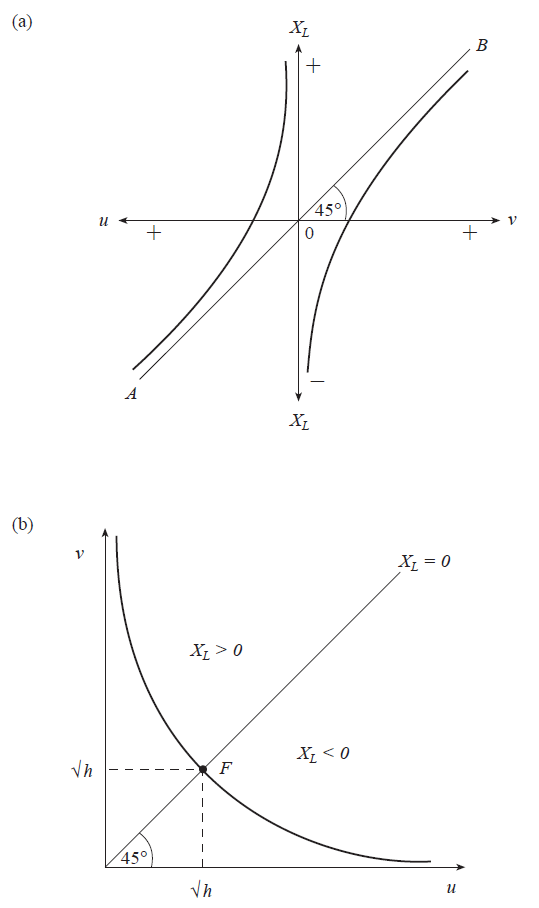
\includegraphics[width=0.25\textwidth]{./figures/aula8_fig5.PNG}}
        \caption{Relação entre excesso de demanda por trabalho, taxas de abertura de vagas e desemprego. Fonte: Snowdon e Vane (2005).}
        \label{fig13}
    \end{figure}
\end{frame}

\begin{frame}{Curva de Phillips}
    \begin{itemize}
        \item Painel (a): quando $X_L$ é zero, as taxas de desemprego e de abertura de postos de trabalho são positivas, refletindo as fricções no mercado de trabalho
        \bigskip
        \item Em um mercado sem fricções, a relação entre $X_L, v$ e $u$ será uma linha de 45º - AB
        \bigskip
        \item Painel (b): combinações de $vu$ em uma curva hiperbólica
        \bigskip
        \item Qualquer ponto ao longo da linha de 45º representa equilíbrio no mercado de trabalho dado que com $X_L = 0$, então, $u = v$
    \end{itemize}
\end{frame}

\begin{frame}{Curva de Phillips}
    \begin{itemize}
        \item O grau existente de fricção no mercado de trabalho é indicado pela posição da curva hiperbólica no ponto $F$: $u = v = \sqrt{h}$
        \bigskip
        \item Um aumento na fricção do mercado de trabalho desloca a curva hiperbólica para a direita
        \bigskip
        \item Este deslocamento, por sua vez, deslocará a curva de Phillips para a direita, dado que o nível de desemprego consistente com $X_L = 0$ aumenta quando a fricção no mercado de trabalho aumenta
        \bigskip
        \item Há forte evidência empírica de que um deslocamento semelhante aconteceu na economia do UK no final dos anos 1960s e começo dos 1970s
    \end{itemize}
\end{frame}

\begin{frame}{Curva de Phillips}
    \begin{itemize}
        \item A relação de Phillips pode, então, ser expressa da seguinte forma:
        \begin{equation}
            \dot{W} = \alpha(h/u - u) + w^* = \alpha h/u - \alpha u + w^*,
            \label{eq9}
        \end{equation}
        onde $w^*$ é um componente de inflação salarial determinado exogenamente (e.g., causado por poder dos sindicatos)
        \bigskip
        \item Note que a inclinação da curva de Phillips depende do coeficiente de flexibilidade dos salários, $\alpha$
        \bigskip
        \item A posição da curva de Phillips, por sua vez, será influenciada por $w^*$ e pelo grau de fricção no mercado de trabalho, $h$
        \bigskip
        \item Quanto mais inflexível o mercado de trabalho (maior $h$), maior será a inflação salarial para qualquer nível de desemprego dado
    \end{itemize}
\end{frame}

\begin{frame}{Curva de Phillips}
    \begin{figure}
        \centering
        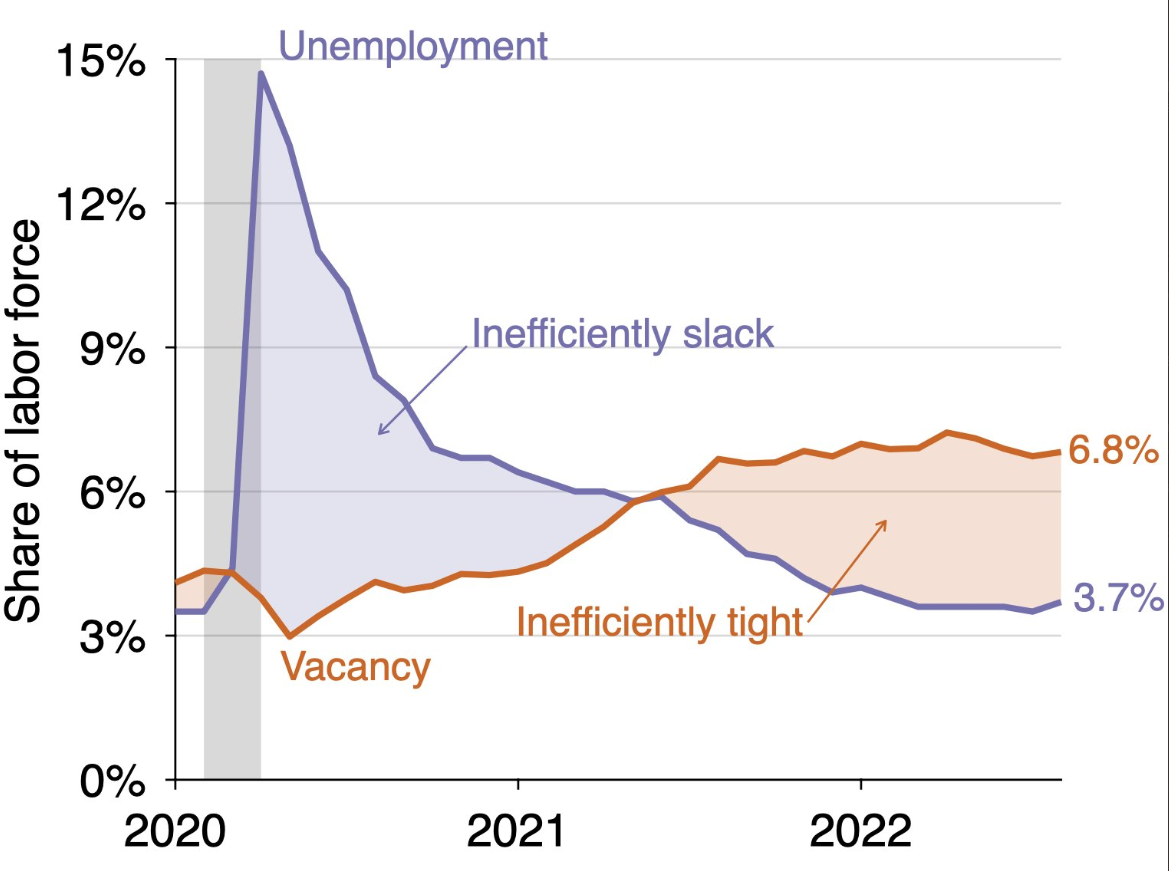
\includegraphics[width=0.6\textwidth]{./figures/aula8_fig6.PNG}
        \caption{Aperto $\times$ folga ineficiente no mercado de trabalho. Fonte: \href{https://pmichaillat.substack.com/p/the-us-labor-market-continues-to}{Michaillat (2022)}.}
        \label{fig:uv}
    \end{figure}
\end{frame}

\begin{frame}{Curva de Phillips}
    \begin{figure}
        \centering
        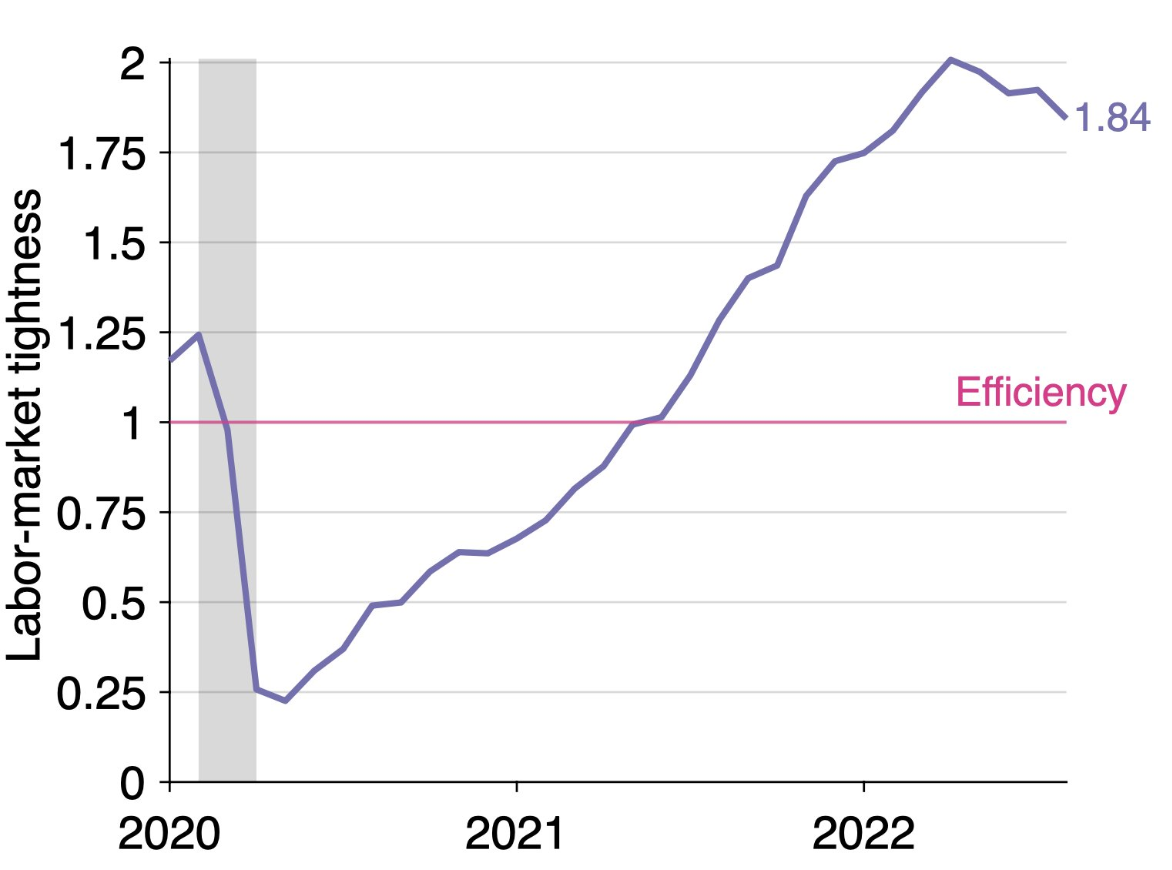
\includegraphics[width=0.6\textwidth]{./figures/aula8_fig7.PNG}
        \caption{Coeficiente de aperto no mercado de trabalho. Fonte: \href{https://pmichaillat.substack.com/p/the-us-labor-market-continues-to}{Michaillat (2022)}.}
        \label{fig:uv}
    \end{figure}
\end{frame}

\begin{frame}{Curva de Phillips}
    \begin{figure}
        \centering
        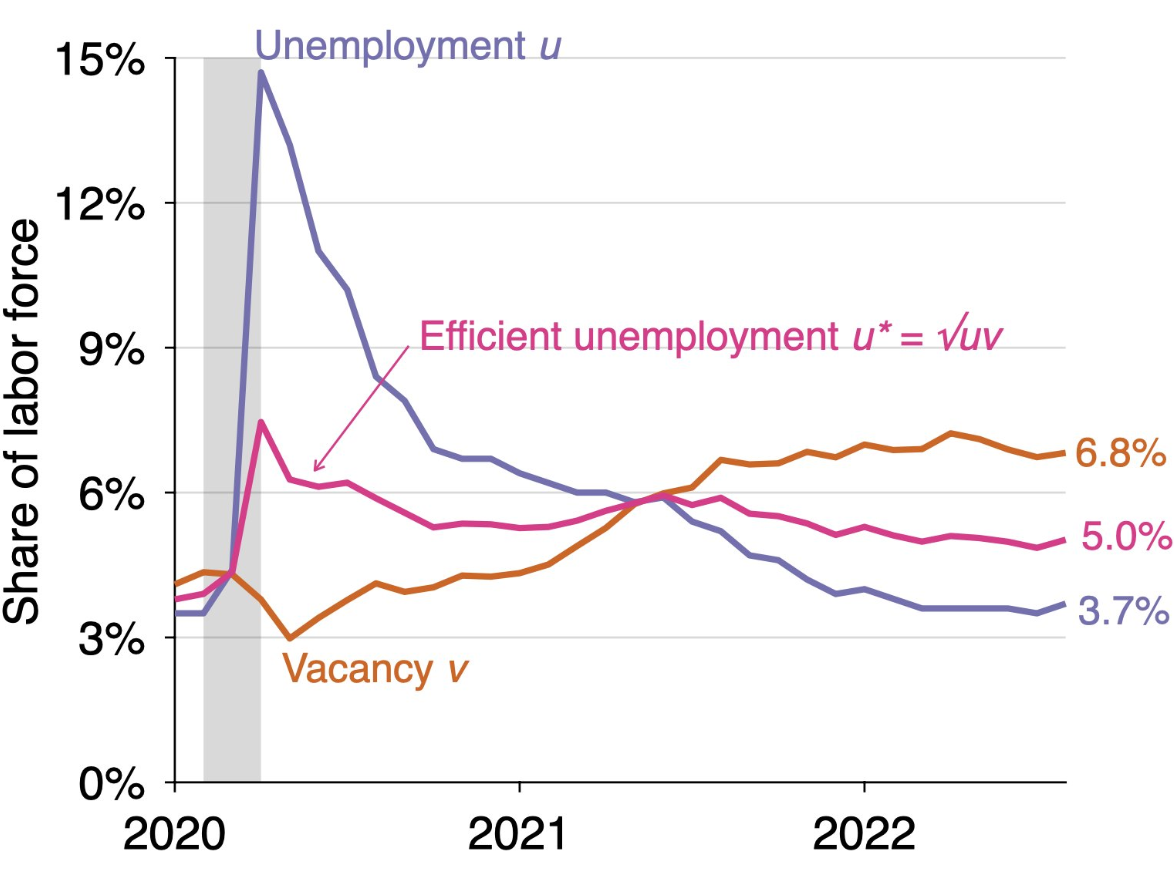
\includegraphics[width=0.6\textwidth]{./figures/aula8_fig8.PNG}
        \caption{Desemprego eficiente. Fonte: \href{https://pmichaillat.substack.com/p/the-us-labor-market-continues-to}{Michaillat (2022)}.}
        \label{fig:uv}
    \end{figure}
\end{frame}

\begin{frame}{Curva de Phillips}
    \begin{itemize}
        \item Década de 1960: rápida incorporação da curva de Phillips ao paradigma ortodoxo Keynesiano
        \bigskip
        \item Até por ser interpretada como implicando um trade-off estável de longo prazo que fornecia aos formuladores de política econômica um menu de combinações possíveis de inflação-desemprego para escolhas de política
        \bigskip
        \item A interpretação de manual da curva de Phillips foi apresentada como uma proposição de que níveis mais baixos de desemprego \emph{permanentes} poderiam ser alcançados se tolerarmos níveis \emph{permanentes} mais elevados de inflação
    \end{itemize}
\end{frame}

\begin{frame}{Curva de Phillips}
    \begin{itemize}
        \item Até final da década de 1960, a ortodoxia Keynesiana usou PC para fazer predições acerca da taxa de inflação que resultaria de diferentes níveis de desemprego obtidas de políticas ativistas de DA, com ênfase em políticas fiscais
        \bigskip
        \item Como DeLong observou, uma vez que estas metas de desemprego continuassem caindo, o resultado inflacionário desta abordagem de política macroeconômica seria inevitável e, de fato, emergiu na grande inflação da década de 1970 - Figura \ref{fig14}
    \end{itemize}
\end{frame}

\begin{frame}{Curva de Phillips}
    \begin{figure}
        \centering
        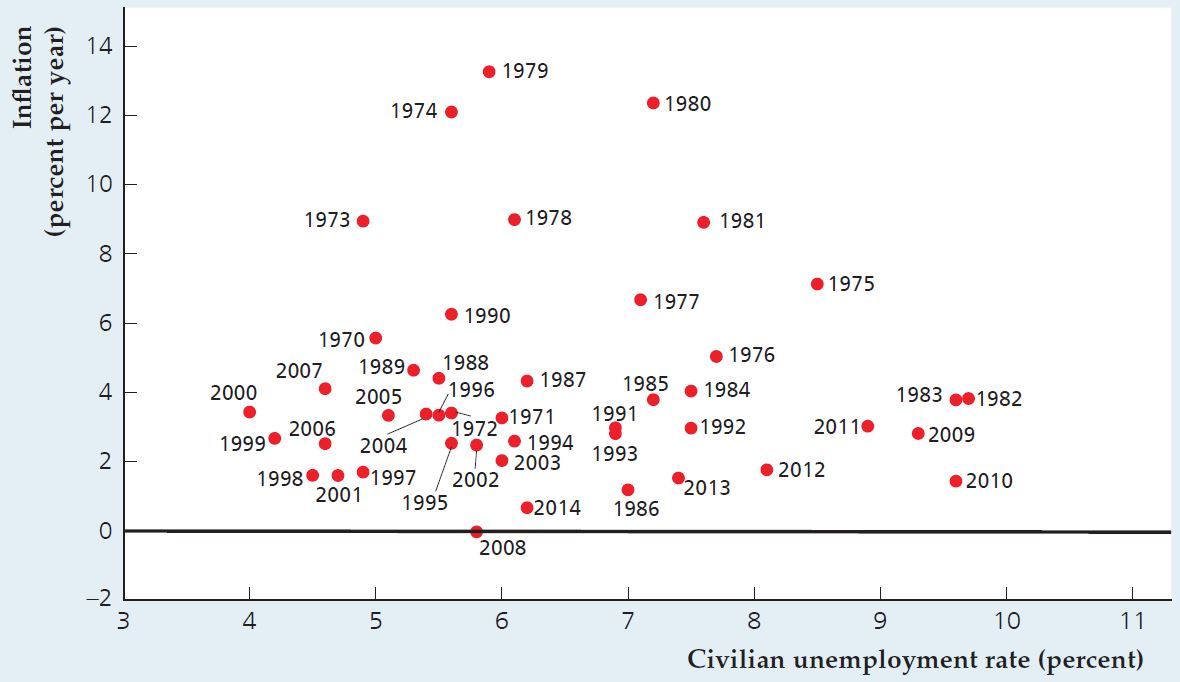
\includegraphics[width=0.7\textwidth]{./figures/aula8_fig9.JPG}
        \caption{Inflação e desemprego nos EUA, 1970 - 2014. Fonte: Abel et al. (2017).}
        \label{fig14}
    \end{figure}
\end{frame}

\begin{frame}{Curva de Phillips}
    \begin{itemize}
        \item Uma das razões para a rápida incorporação da PC aos modelos Keynesianos ortodoxos é que parecia fornecer uma explicação para a determinação da inflação que estava ausente nos modelos macro vigentes
        \bigskip
        \item A hipótese adotada no modelo IS-LM (Macro I) era de que o nível de preços era fixo em um valor abaixo do compatível com o pleno emprego, com o resultado de que até o nível de pleno emprego, variações na DA afetam o nível de renda real e de emprego
    \end{itemize}
\end{frame}

\begin{frame}{Curva de Phillips}
    \begin{itemize}
        \item Com rigidez de salários nominal, até o valor de pleno emprego, salários nominais são fixos e, portanto, não respondem a variações de DA
        \bigskip
        \item Apenas quando a economia atingia pleno emprego que variações de DA afetam o nível de preços
        \bigskip
        \item A curva de Phillips possibilitou que a teoria Keynesiana ortodoxa de determinação do produto e do emprego fosse combinada com uma teoria da inflação de preços e salários
    \end{itemize}
\end{frame}

\begin{frame}{Curva de Phillips}
    \begin{figure}
        \centering
        \href{https://raw.githubusercontent.com/pvfonseca/pec/main/notas/figures/aula8_fig10.PNG}{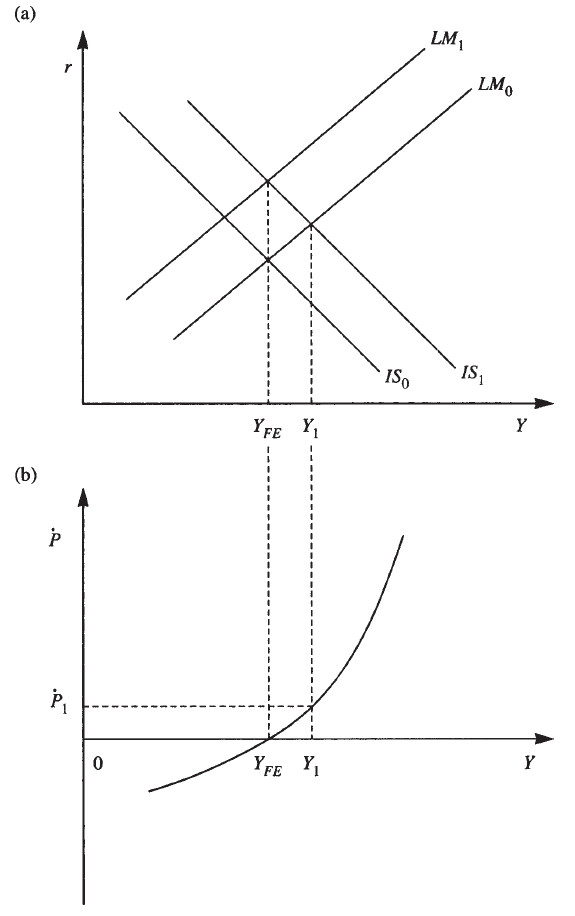
\includegraphics[width=0.25\textwidth]{./figures/aula8_fig10.PNG}}
        \caption{Modelo IS-LM e curva de Phillips. Fonte: Snowdon e Vane (2005).}
        \label{fig15}
    \end{figure}
\end{frame}

\begin{frame}{Curva de Phillips}
    \begin{itemize}
        \item Figura \ref{fig15} (Lipsey, 1978): modelo IS-LM no painel (a) e a curva de Phillips no painel (b) - com inflação de preços $\dot{P}$ e renda $Y$ nos eixos
        \bigskip
        \item O painel (b) é derivado sob as seguintes hipóteses:
        \bigskip
        \begin{enumerate}
            \item O nível de produto depende do nível de emprego e o nível de desemprego é inversamente relacionado com o nível de emprego
            \bigskip
            \item Os preços são determinados com um mark-up sobre os custos unitários da produção, cujo principal componente é o salário
        \end{enumerate}
        \bigskip
        \item A hipótese de um mark-up sobre o custo unitário da produção sugere que a inflação de preços depende da inflação de salário nominal menos o crescimento da produtividade
    \end{itemize}
\end{frame}

\begin{frame}{Curva de Phillips}
    \begin{itemize}
        \item Na curva de Phillips estimada que vimos, um nível de desemprego de $\approx 2,5\%$ era compatível com estabilidade de preços
        \bigskip
        \item Isso porque, a este nível de desemprego, a taxa de variação do salário nominal era aproximadamente igual ao crescimento médio da produtividade - que era de 2\%
    \end{itemize}
\end{frame}

\begin{frame}{Curva de Phillips}
    \begin{itemize}
        \item Com relação à Figura \ref{fig15}, notamos que o nível de renda de pleno emprego é compatível com estabilidade de preços ($\dot{P} = 0$)
        \bigskip
        \item Uma expansão fiscal permanente desloca a curva IS para a direita, fazendo com que o produto agregado aumente para um nível maior que o de pleno emprego
        \bigskip
        \item Pela curva de Phillips, à medida que a renda aumenta para valores acima do de pleno emprego, a inflação de preços cresce
        \bigskip
        \item O aumento da inflação de preços reduz o valor real da oferta monetária - deslocando a curva LM para a esquerda
        \bigskip
        \item Este processo de ajuste continuará até a economia retornar para o equilíbrio de pleno emprego
    \end{itemize}
\end{frame}

\section{Bibliografia}
\begin{frame}{\emoji{books} Bibliografia}
    \begin{itemize}                        
        \item ABEL, A.; BERNANKE, B.; CROUSHORE, D. Macroeconomics. 9.ed. Pearson Prentice Hall, 2017\medskip
        \item BLANCHARD, O. Macroeconomia. 7.ed. São Paulo: Pearson Education do Brasil, 2017\medskip
        \item DORNBUSCH, R.; FISCHER, S.; STARTZ, R. Macroeconomia. 11.ed. Porto Alegre: AMGH, 2013 \medskip
        \item HANSEN, B. Excess Demand, Unemployment, Vacancies and Wages, Quarterly Journal of Economics, February, 1970\medskip
        \item LIPSEY, R.G. The Relationship Between Unemployment and the Rate of Change of Money Wage Rates in the U.K. 1862–1957: A Further Analysis, Economica, February, 1960\medskip
        \item LIPSEY, R.G. The Place of the Phillips Curve in Macroeconomic Models, in A.R. Bergstrom (ed.), Stability and Inflation, Chichester: John Wiley, 1978\medskip
        \item MICHAILLAT, P.; SAEZ, E. \href{https://pascalmichaillat.org/13.pdf}{$u^* = \sqrt{uv}$}, 2023\medskip
        \item PHILLIPS, A.W. The Relation Between Unemployment and the Rate of Change of Money Wage Rates in the United Kingdom, 1861–1957, Economica, November, 1958\medskip
        \item SNOWDON, B.; VANE, H.R. \emph{Modern Macroeconomics: its Origins, Development and Current State}. Northampton, MA: Edward Elgar, 2005\medskip        
    \end{itemize}
\end{frame}
\end{document}